\documentclass{article}
\usepackage{amsmath}
\usepackage[utf8]{inputenc}
\usepackage{natbib}
\bibliographystyle{abbrvnat}
\setcitestyle{authoryear,open={((},close={))}}
\usepackage{graphicx}
\usepackage{float}
\usepackage[margin=1in]{geometry}
\usepackage[framed,numbered,autolinebreaks,useliterate]{mcode}

\title{MTH 5315 NUMERICAL METHODS FOR PDE \\ MIDTERM 2}

\date{\today}
\author{\Huge Max Le \\ \\ ID: 901223283}
\begin{document}
\maketitle
\newpage
\tableofcontents
\newpage
\listoffigures

\newpage
\section{Introduction}
For this midterm, we are given the following 1D-Poisson equation to solve:

\begin{equation}
u_{xx} = 1-2x^2 \textrm{ on the domain (0,1)}
\end{equation}

\noindent
with Dirichlet boundary conditions as follow: $u(0) = u(1) = 0$. The problem is to be solved using until a relative residual error of $10^{-5}$ is achieved at a grid size of 128.The results are plotted and the convergent analysis is performed for each case. An analytical solution is also obtained via the following procedure:
\begin{align*}
u_{xx}(x) &= 1-2x^2 \\
\dfrac{d}{dx}(u_x(x))&= 1-2x^2\\
u_x(x)&= \int_{0}^{x} (1-2x^2) dx\\
&=x-\dfrac{2x^3}{3}+C1\\
u(x) &= \int_{0}^{x} (x-\dfrac{2x^3}{3}+C1) dx\\
&=\dfrac{x^2}{2} - \dfrac{x^4}{6} + C1x + C2\\
\end{align*}
\noindent
Applying the boundary conditions:

\begin{align*}
u(x) &=  \dfrac{x^2}{2} - \dfrac{x^4}{6} - \dfrac{x}{3}
\end{align*} The 2nd derivative is discretized using a 2nd order central difference scheme as follow: 

\begin{equation}
U_{xx} \approx \dfrac{U_j-2U_j+U_j}{\Delta x^2} + O(\Delta x^2)
\end{equation}

\noindent
This finite difference equation, when combine together with our original PDE, can be written in the form of a linear algebra system, $Au = f$: 

\[
\dfrac{1}{\Delta x^2}\begin{bmatrix}
-2 & 1 & 0 & \dots & 0 \\
1 & -2 & 1 & \dots & 0 \\
0 & 1 & -2 & 1 & \dots \\
\dots  & \dots  & \dots  & \dots & \dots  \\
\dots & \dots & \dots & \dots & \dots 
\end{bmatrix}
\begin{bmatrix}
u_1 \\ u_2 \\ u_3 \\ \dots \\ u_n 
\end{bmatrix}
=
\begin{bmatrix}
f_1 \\ f_2 \\ f_3 \\ \dots \\ f_n 
\end{bmatrix}
\]

\noindent
With the Dirichlet boundary conditions, our values for $f_1$ and $f_n$ are 0. There are no need to include ghost points; therefore, our revised linear system is follow: 

\[
\dfrac{1}{\Delta x^2}\begin{bmatrix}
-2 & 1 & 0 & \dots & 0 \\
1 & -2 & 1 & \dots & 0 \\
0 & 1 & -2 & 1 & \dots \\
\dots  & \dots  & \dots  & \dots & \dots  \\
\dots & \dots & \dots & \dots & \dots 
\end{bmatrix}
\begin{bmatrix}
u_1 \\ u_2 \\ u_3 \\ \dots \\ u_n 
\end{bmatrix}
=
\begin{bmatrix}
0 \\ f_2 \\ f_3 \\ \dots \\ 0 
\end{bmatrix}
\]

\section{Jacobi Relaxation}
\subsection{About the method}
The general form for an iterative method to solve $Au = f$ is: 

\begin{equation}
	U^{k+1} = (I-B^{-1}A)U^k+B^{-1}f
\end{equation}
\noindent
Where I = identity matrix, D = diagonal vector of A. Also recall that for Jacobi: $B = D^{-1}$, the Jacobi iterative method is as follow: 

\begin{equation}
	U^{k+1} = (I-D^{-1}A)U^k+D^{-1}f
\end{equation}
\noindent
In order to include the under-relaxation feature, the equation needs to be rewitten. The Jacobi method with relaxation parameter, $\omega$, is written as follow:

\begin{equation}
	U^{k+1} = \omega[(I-B^{-1}A)U^k+B^{-1}f] + (1-w)IU^k
\end{equation} 
\noindent
For our problem, $\omega$ is taken to be 0.75. 

\subsection{Results}




Below are results for this method, we have the results converged at 48,906 iterations. 

\begin{figure}[H]
	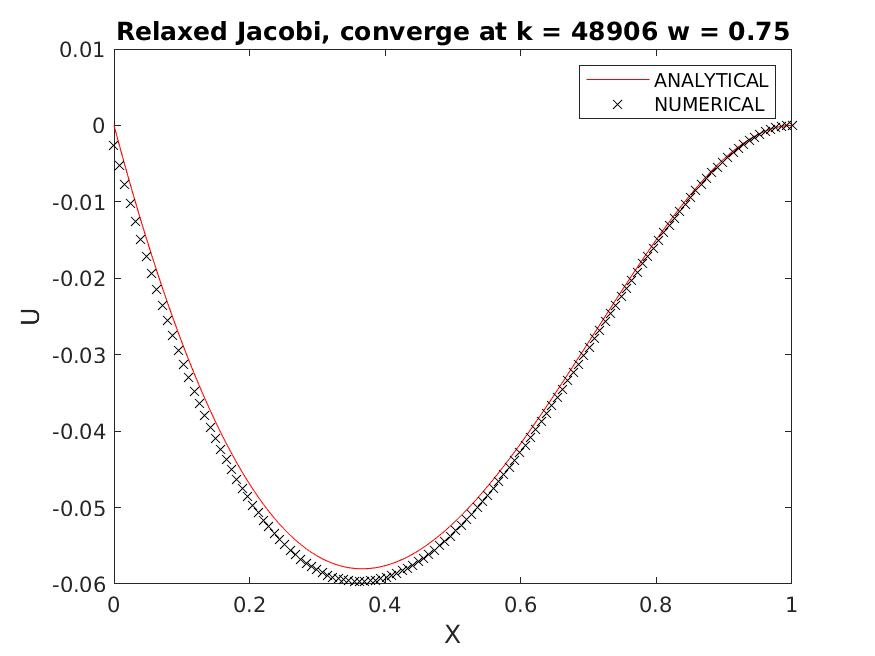
\includegraphics[width=\linewidth]{jacobi75.jpg}	
	
	\caption{Analytical vs Numerical for Under Relaxed Jacobi for w = 0.75}
\end{figure}

\begin{figure}[H]
	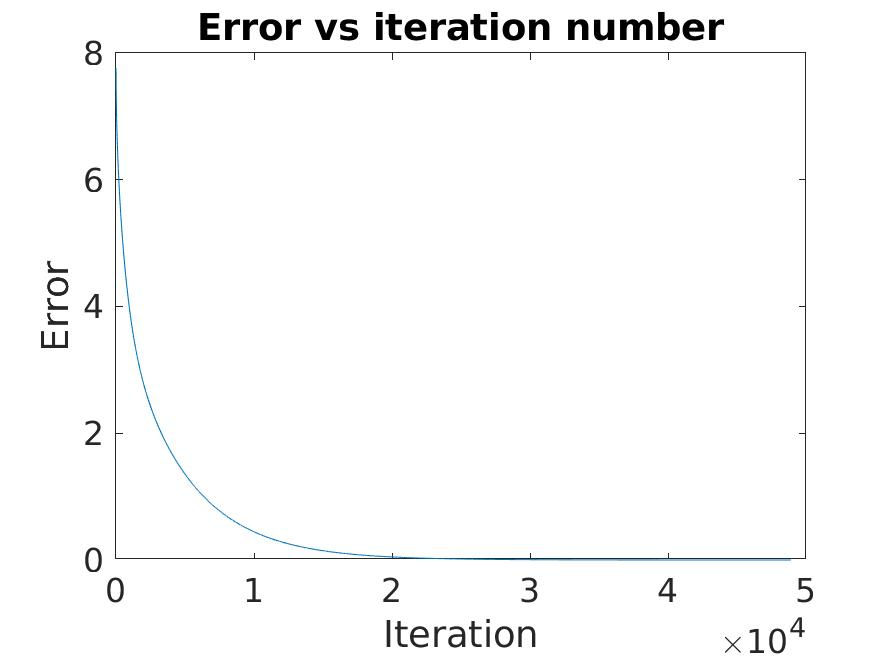
\includegraphics[width=\linewidth]{jacobi_error.jpg}	
	
	\caption{Error vs iteration number for w = 0.75}
\end{figure}

\subsection{Analysis}

The Jacobi method is known to be very slow; in this case, we added an under-relaxed parameter, which makes it even slower. The scheme needs almost 60,000 iterations to converge to the analytical solution.  Writing in standard form   
\begin{align*}
	U^{k+1}&=Ru^k+c\\
	&=\left(\omega(I-D^{-1}A+(1-\omega)I)\right)U^{k} + wD^{-1}f
\end{align*}

\noindent
The iterative matrix,R, of this method is as follow: 

\begin{equation}
	R = \omega(I-D^{-1}A)+(1-\omega)I
\end{equation}

\noindent
From class notes, for the iterative method to converge, then $||R|| < 1$. Also recall that if R is symmetric then the 2-norm should be used to test for convergence. In this problem, the matrix R looks something like this: 
\[
\begin{bmatrix}
	0.25 & 0.375 & 0 & \dots & 0 \\
	0.375 & 0.25 & 0.375 & \dots & 0 \\
	0 & 0.375 & 0.25 & \dots & \dots \\
	\dots  & \dots  & \dots  & \dots & \dots  \\
	\dots & \dots & \dots & \dots & \dots 
\end{bmatrix} 
\]

\noindent
Its transpose is also the same, therefore we need to use a 2-norm to determine the convergence of this method. This is done by taking the square root of the sum of the squares of all the elements. In the code, the function \textbf{norm} is used and it gives the answer of \textbf{0.998} which is less than 1. Therefore, we can say that this method always converges. Another way to determine convergence is to compute the eigenvalue of R. We can think of the Under Relax Jacobi as a normal Jacobi with some deviations (caused by the relaxation parameter $\omega$). In class, the k-th eigenvalue is computed and it is as follow: 

\begin{equation}
	\lambda_k = cos\left(\dfrac{k\pi}{N+1}\right) \textrm{ , k =1,2,...,N}
\end{equation}

\noindent
From trigonometry, cosine is bounded by 1; therefore, $cos\left(\dfrac{k\pi}{N+1}\right)$ is always bounded 1 and therefore always converges.
The convergence rate of the method is dictated by how quickly $||R||$ goes to zero. For an iterative method: 

\begin{align*}
	e^k &= x - x^k\\
	 &= Re^{k-1} = R(Ae^{k-1}) = ... = R^ke^{(0)}
\end{align*} 
 
\noindent
This can be understood as: the error at after k-th iteration is governed by the value of the matrix R and the initial error.  If the 2-norm is taken, then $||e^k|| = ||R^ke^{(0)}|| = ||R^k||*||e^{(0)}||$. The convergence rate is therfore controlled by $||R^k||$, which is found out to be \textbf{0.998}, which is also $\rho$- the spectral radius. One thing we can say is that the error rate drops very slow after 1 iteration: 

\begin{equation*}
	\textrm{Error rate drop} = 1- 0.998 = 0.002 = 0.2\%
\end{equation*}

\noindent
Therefore, the Under Relaxed Jacobi, when applies to this problem, gives converged solution.  However, the rate of convergence is very slow. We need at least 60,000 iterations to satisfy a tolerance of $10^{-5}$. As an additional investigation, if the value of $\omega$ is changed, then we have: 

\begin{figure}[H]
	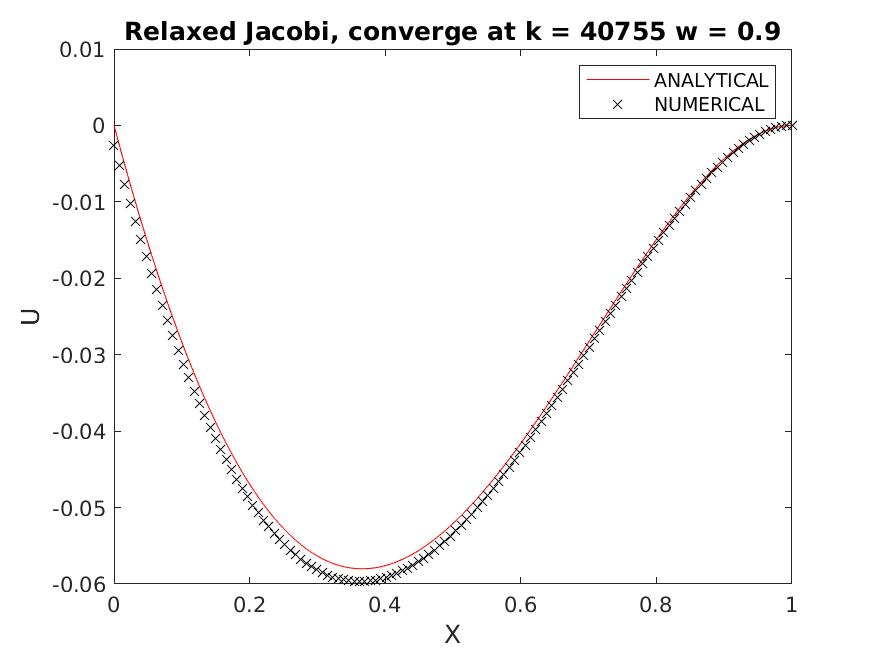
\includegraphics[width=\linewidth]{jacobi90.jpg}	
	
	\caption{Analytical vs Numerical for Under Relaxed Jacobi for w = 0.9}
\end{figure}

\noindent
Clearly,the number of iterations decrease as $\omega$ goes up. However, if we keep increasing: 

\begin{figure}[H]
	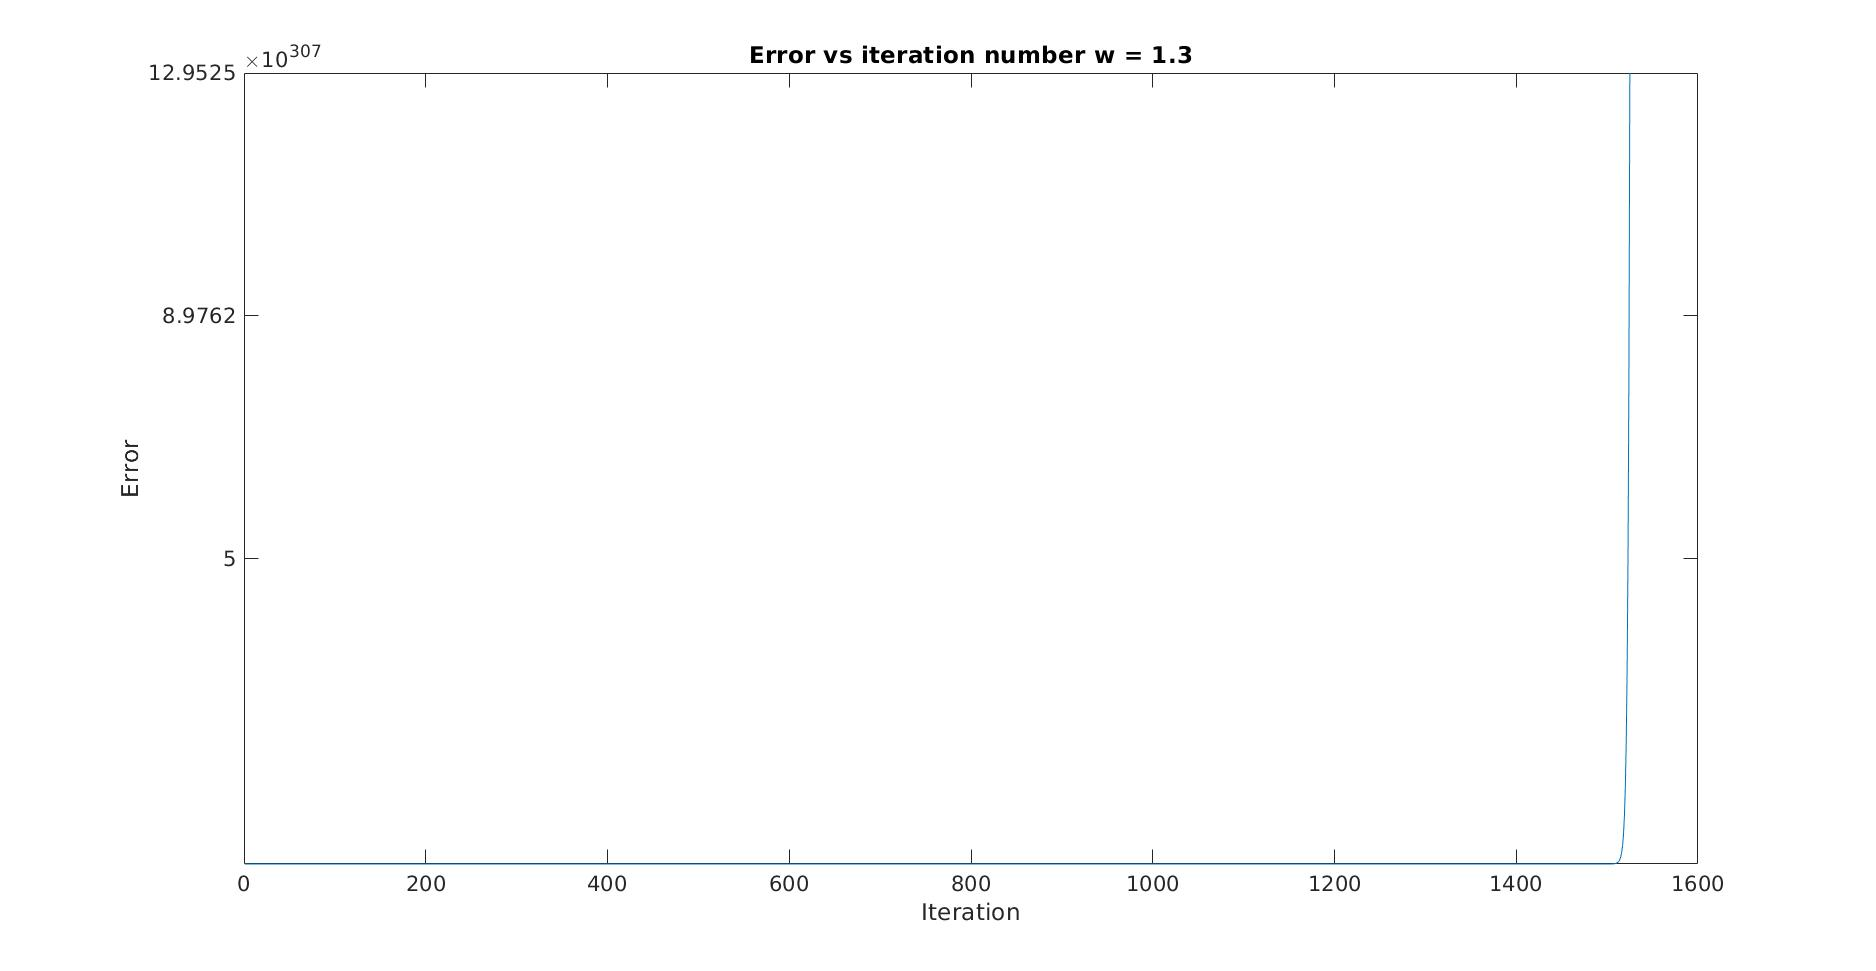
\includegraphics[width=\linewidth]{jacobi_error_blow.jpg}	
	
	\caption{Error vs iteration number for w = 1.3}
\end{figure}

\noindent
The error blows up too much that the scheme is unable to find a converge solution. In our error equation, the iterative error term $e^k$ is too large for the iterative matrix $R^k$ and the initial error $e^{(0)}$ to contain and reduce. 


\section{Multigrid V-Cycle}
\subsection{About the method}
The basic idea of the Multigrid method is to remove errors at low frequencies. Gauss-Seidel and Jacobi method and their error vector,e, has most of the high frequency errors removed but not the low frequency ones. These errors are usually not removed because they are in the "smooth" region. In order to do this, we change from a fine grid to a coarser grid, such that smooth errors become rough errors and as a result, the low frequency errors will appear as high frequency errors and hopefully, will be removed by the usage of Gauss-Seidel/Jacobi.. After the errors are removed, we then convert the coarser grid back into the fine grid and get our results. This "return step" is done by an interpolation matrix $I_{2h}^{h}$. \\

\noindent
Our problem requires a 4 level of grid coarsening V-cycle multigrid. As a result, the top "fine" grid will have 128 elements, the next coarse grid will have 64, then 32, then 16 and 8 elements. A visual for this V-cycle method can be shown below: 

\begin{figure}[H]
	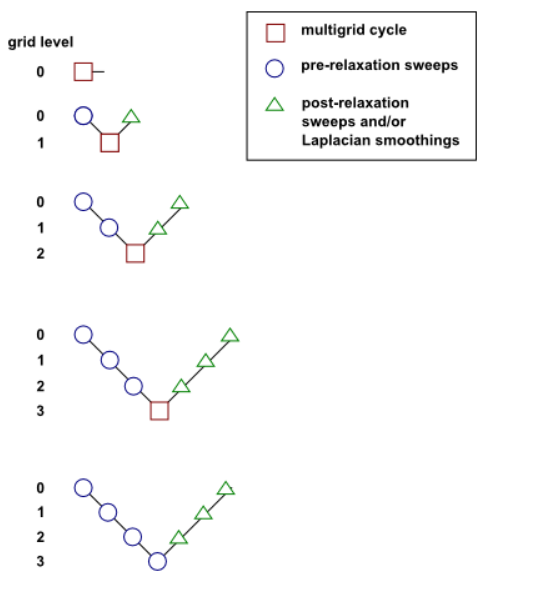
\includegraphics[width=\linewidth,height = 150mm]{multigrid.png}		
	\caption{Error vs iteration number}
\end{figure}



\newpage
\subsection{Results}
Below are the results obtained for this method. We have convergent at 21 iterations. 

\begin{figure}[H]
	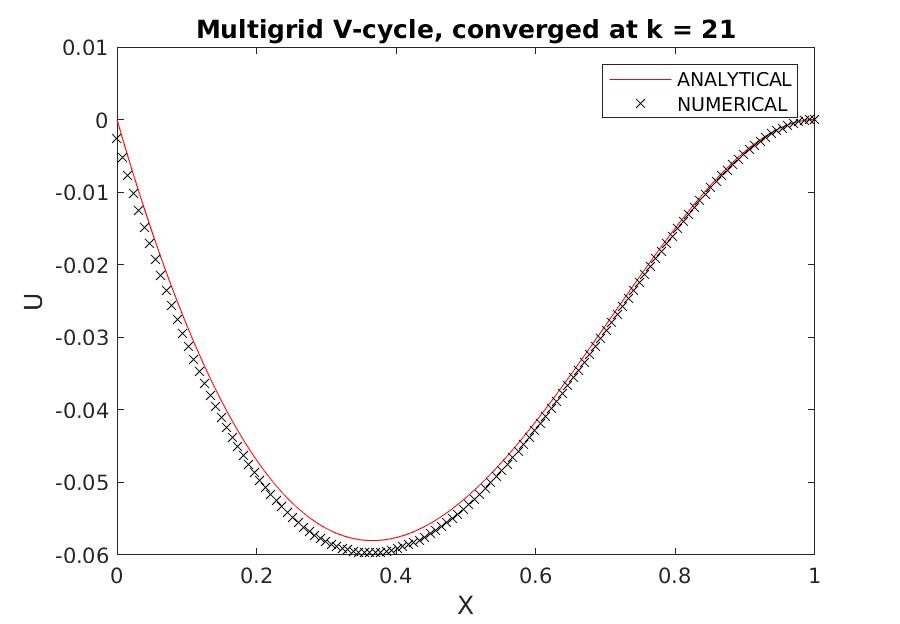
\includegraphics[width=\linewidth]{vcycle.jpg}	
	\caption{Analytical vs Numerical for 4-Level V-cycle Method}
\end{figure}

\begin{figure}[H]
	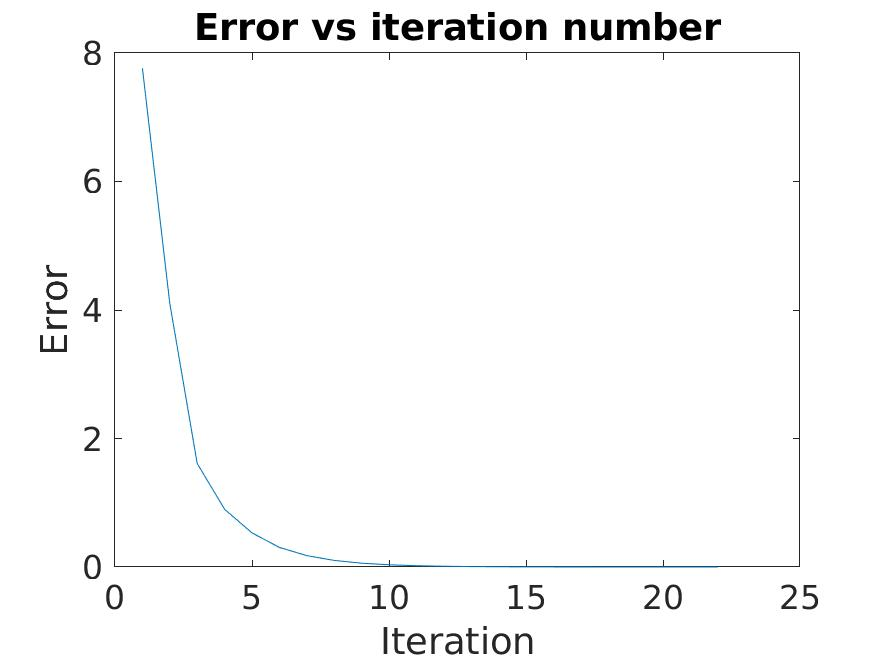
\includegraphics[width=\linewidth]{vcycle_error.jpg}	
	\caption{Error vs Iteration number for 4-Level V-cycle Method}
\end{figure}


\subsection{Analysis}

It can be seen that the Multigrid approach is extremely efficient. From before, we need almost 60,000 iterations to converge.  Now, we only need around 10 iterations to converge. A similar analysis containing the kth level error and initial error can also be done: 

\begin{equation}
	e^{k} \leq \rho e^{0}
\end{equation} 
\noindent
Where $\rho$ is the constant factor to govern the convergence rate of the method that is independent of the grid size. In the code, this $\rho$ is calculated to be: \textbf{$1.22*10^{-6}$}.  This is significantly smaller than the value we calculated for Jacobi, which was 0.999. Using the same analysis, after 1 iteration, the error gets reduced by: $1-1.22*10^{-6} = 0.99999878 = 99.9\%$.  These are all estimates because rigorous analysis of the convergence rate are not discussed in class. However, it still give us an idea of how fast and efficient the Multigrid V-cycle method is. 

\begin{figure}[H]
	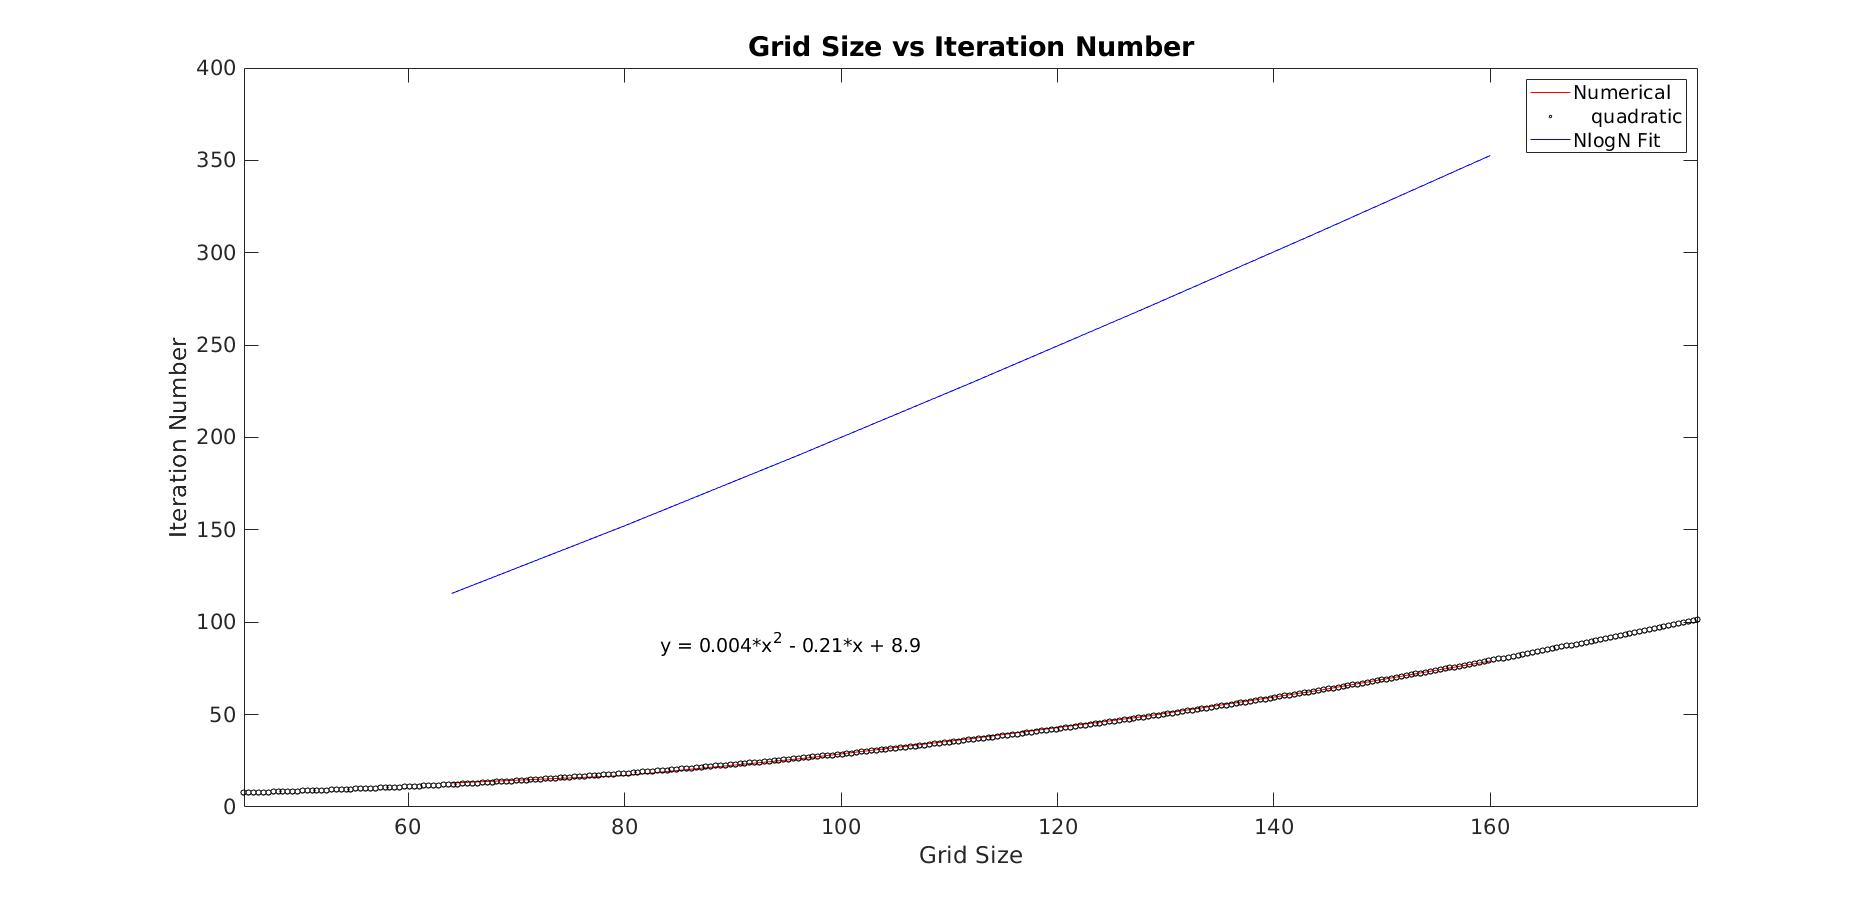
\includegraphics[width=\linewidth]{gridsize_iter.jpg}	
	\caption{Grid Size vs Iteration number for 4-Level V-cycle Method}
\end{figure}

\noindent
The plot above shows the grid size vs the number of iteration it needs to converge for our particular problem. It can be seen as grid size increases, we need more iterations. This is understandable because the larger problem contains more unknowns and therefore more equations are needed to be solved. Theoretically, the curve $NlogN$ can be used to fit our numerical data.  However, this is only estimate because we have not really covered the diffrent parameters such as y-intercept,x-intercept of the $NlogN$ curve for this method. Instead, another polynomial curve is fitted to show the general trend. This is a 2nd order polynomial and if we think about it, the result makes sense.  The reason for this is that our original PDE is discretized using a 2nd order central difference with a local truncation error of $\Delta x^2$. Therefore, if we "square" our gridsize, then the error should also increase which makes the number of iterations needed to also increase. They will following a 2nd order polynomial curve ($x^2$)

\section{Conclusion}
In conclusion, the Under Relaxed Jacobi method shows how the value of the relaxation parameter, $\omega$, is important in controlling the convergence rate. Good choice of $\omega$ will speed up the convergence rate;however, poor choice of $\omega$ will cause the numerical solution to blow up. On the other hand, the Multigrid V-cycle involves a recursive algorithm to take care of the errors at low frequency. This is done by mapping the problem from an original (fine) grid to a coarser grid, with the hope that the errors at low frequency becomes high frequency and therefore can be reduced by the usage of Jacobi/Gauss-Seidel..etc. The result was significantly better than Under Relaxed Jacobi, we managed to get a much lower iteration numbers to satisfy the same tolerance.  From the error plots, we can also see clearly how the errors for the V-cycle drop to around 0 after 5 iterations, compare to Under Relax Jacobi, where the we need at least 20,000 iterations to get a "low" error.  Finally, the comparison between Grid Size and Iteration Number shows how the scheme follows a quadratic increase in terms of iteration number and error.  If more info is given, then the curve $NlogN$ can be fitted better to show that the scheme follows an $NlogN$ order. 

\newpage
\section{Matlab Codes}
\subsection{Under Relaxed Jacobi}
\lstinputlisting{relax_sor.m}
\newpage
\subsection{Multigrid V-Cycle}
\lstinputlisting{v_cycle.m}


\end{document}
